%!TEX root = ../main.tex

\chapter{\label{ch:feats}Basic template features}

I assume you already know how to use \LaTeX, so I won't write a lot.
Some \emph{words} are more important than others, so you might want to \emph{emphasize} them with the \texttt{\textbackslash emph} command.
On the other hand, you might wanna tell more about something without taking up a lot of space in the main text.
That's when you use footnotes\footnote{Just use the command \texttt{\textbackslash footnote}...}!

In a good scientific text, it is crucial to cite other people's work. If you say something important, make sure to \texttt{\textbackslash cite} it soon afterward \cite{10.1088/1367-2630/ad313e}. By the way, Ref.~\cite{10.1088/1367-2630/ad313e} is not saying anything useful to this purpose, so don't look at it. The bibliography entries are located in \texttt{refs.bib}.




\section{Math}

An equation might look like this $\mathcal{H}(\lambda) = A(t)\mathcal{H}_{A} + B(t)\mathcal{H}_{B}$, if inline. 
Otherwise, you might take more space:
\begin{equation*}
    \mathcal{H}(\lambda) = A(t)\mathcal{H}_{A} + B(t)\mathcal{H}_{B} + C(t)\mathcal{H}_{C} + ...
\end{equation*}

I will put here more math stuff with equations, just to make my point. Let $\ket{\psi(t)}$ be a quantum state that evolves in the time interval $[0,\tau]$. Its dynamics are described by the time-dependent Schrödinger equation.
$$i\ket{\dot\psi(t)} = \mathcal{H}(t)\ket{\psi(t)}$$
We use from now on the natural units $\hbar=1$. Let us introduce the basis of instantaneous eigenstates $\ket{n(t)}$ with eigenvalues $\epsilon_n(t)$:
\begin{equation}
    \label{eq:adth-eigenvalue}
    \mathcal{H}(t)\ket{n(t)} = \epsilon_n(t) \ket{n(t)}
\end{equation}
Since $\{\ket{n(t)}\}$ is a complete orthonormal set, $\ket{\psi(t)}$ can be expressed as a linear combination in that basis:
\begin{equation}
    \ket{\psi(t)} = \sum_n c_n(t) e^{i\theta_n(t)} \ket{n(t)}
\end{equation}
We have explicitly factorized the phase $\theta_n(t)=\int_0^t \epsilon_n(t')dt'$ from $c_n(t)$. This choice will be convenient in the following calculations, but it can be intuitively motivated straight away. 
It is known that an eigenstate picks up a phase $e^{-i\epsilon_n}$ when it evolves under a constant Hamiltonian. The $\theta_n(t)$ is a generalization of the picked-up phase, obtained by integrating it throughout the time interval in which the Hamiltonian evolves. It is known as the Berry phase.\\


To show the use of \texttt{\textbackslash underbrace\{\}}, we now write the Schrödinger equation in a rotating frame:
\begin{align}
    i\frac{d\ket{\tilde{\psi}}}{dt} &= i\left( \frac{dU^\dag}{dt}\ket{\psi} + U^\dag \frac{d\ket{\psi}}{dt} \right) = \nonumber\\
    &= i\dot\lambda \partial_\lambda U^\dag \cdot U\ket{\tilde{\psi}} + U^\dag\mathcal{H}\cdot U\ket{\tilde{\psi}} =\nonumber\\
    & \equiv \underbrace{\left( \tilde{\mathcal{H}} - \dot\lambda \tilde{\mathcal{A}}_\lambda \right)}_{\mathcal{H}_{rot}}\ket{\tilde{\psi}} \label{eq:schr-movingframe}
\end{align}

Just a suggestion: define recurrent symbols in \texttt{custom-symbols.tex}. For instance, typing \texttt{\textbackslash hamCD} to print $\hamCD$ is way more compact than typing
\begin{center}
    \texttt{\textbackslash mathcal\{H\}\_\{\textbackslash mathrm\{CD\}\}}
\end{center}
all the time...





\subsection{Theorem support}

You might input some theorem!

\begin{theorem}
Suppose that the spectrum of $\mathcal{H}(\lambda)$ has the ground state eigenvalue separated by a gap $\Delta(\lambda)=\epsilon_1(\lambda)-\epsilon_0(\lambda)\ >0$ from the rest of the spectrum, and that $\mathcal{H}$ is twice continuously differentiable. Assume that $\mathcal{H}$, $\partial_\lambda\mathcal{H}$ and $\partial^2_\lambda\mathcal{H}$ are bounded operators (an assumption that is always fulfilled in finite-dimensional spaces). Then
\begin{equation}
    \tau \gg \max\left(
        \max_\lambda \frac{\|\partial_\lambda\mathcal{H}(\lambda)\|}{\Delta^2(\lambda)},
        \max_\lambda \frac{\|\partial^2_\lambda\mathcal{H}(\lambda)\|}{\Delta^2(\lambda)}, 
        \max_\lambda \frac{\|\partial_\lambda\mathcal{H}(\lambda)\|^2}{\Delta^3(\lambda)}
    \right) .
\end{equation}
\end{theorem}








\section{Glossary}

In \texttt{docs/glossary.tex}, one might introduce acronyms that are printed in the table at the end of the document. The syntax is simple:

\begin{center}
    \texttt{\textbackslash newacronym\{acronym-label\}\{EAT\}\{Extended Acronym Text\}}
\end{center}

To reference the acronym, use the command \texttt{\textbackslash gls}. 
In the previous example, the command \texttt{\textbackslash gls\{acronym-label\}} will print:
\begin{itemize}
    \item \gls{acronym-label}, if the acronym has not been used before.
    \item \gls{acronym-label}, if the acronym has already been used in the text.
    \item Here, \gls{acronym-label} has been called for the third time!
\end{itemize}

It is possible to reset the counter for all the acronyms with \texttt{\textbackslash glsresetall}, or to reset the counter for a specific acronym with \texttt{\textbackslash glsreset\{acronym-label\}}.




\section{References and floating objects}

Using the \texttt{\textbackslash ref} command, you might reference labeled objects.
Chapter~\ref{ch:feats} is the only useful chapter of this template.
All the others, in Part~\ref{prt:filler}, are just filled with \texttt{lipsum} text.
The appendices are referenced with letters: for instance Appendix~\ref{ax:demo}.\\

When referencing equations, it is recommended to use \texttt{\textbackslash eqref} instead. 
For instance, Eq.~\eqref{eq:adth-eigenvalue} is clearly understood by any physics undergraduate!\\

Tables in \LaTeX are quite nice! Take a look at Table~\ref{tab:demo}.\\

\begin{table}[h]
\centering
\begin{tabular}{c|c|cc|cc}
    &\multirow{2}{*}{UA}&\multicolumn{2}{c|}{CD}&\multicolumn{2}{c}{FE}\\
    &&$\ell=1$&$\ell=2$&$\ell=1$&$\ell=2$\\\hline
    $f(\tau) \;[10^{-2}]$&1.5793&7.4970&17.039&7.5554&17.162\\
    $m(\tau)$&0.50107&0.69264&0.80038&0.69354&0.80143\\
    \hline
\end{tabular}
\caption{\label{tab:demo}Fidelity and energy merit resulting from an annealing simulation.}
\end{table}



Another kind of floating object are, of course, figures! To keep it simple, look at Figure~\ref{fig:demo}.\\

\begin{figure}
    \centering
    \includegraphics[height=6cm]{example-image-a}
    \caption{Simple example of floating image demo.}
    \label{fig:demo}
\end{figure}


As for plots, I recommend you save them in PDF format (Figure~\ref{fig:demo-plot}).

\begin{figure}
    \centering
    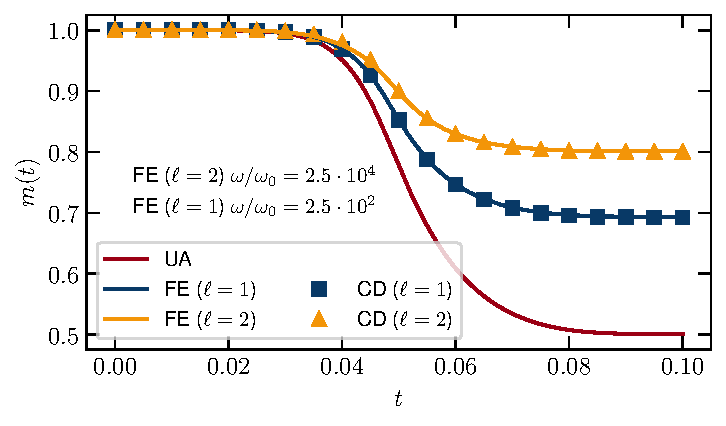
\includegraphics[height=7cm]{img/demo-plot.pdf}
    \caption{Simple example of plot saved in PDF and imported in the document. As you see, it is all vectorized!}
    \label{fig:demo-plot}
\end{figure}


\lipsum[1-5]






\section{Drawing with tikz}

When you get skilled, you might want to create drawings in \texttt{tikz}, like in Figure~\ref{fig:demo-max-cut}.
You can make equations with drawings,
% note: this is an equation with drawings\
%
% Gradient Info
\tikzset {_2wjvdlgsv/.code = {\pgfsetadditionalshadetransform{ \pgftransformshift{\pgfpoint{0 bp } { 0 bp }  }  \pgftransformrotate{-45 }  \pgftransformscale{2 }  }}}
\pgfdeclarehorizontalshading{_189nw8o3l}{150bp}{rgb(0bp)=(0.03,0.22,0.4);
rgb(37.5bp)=(0.03,0.22,0.4);
rgb(43.86904580252511bp)=(0.03,0.22,0.4);
rgb(62.5bp)=(0.05,0.36,0.63);
rgb(100bp)=(0.05,0.36,0.63)}
\tikzset{every picture/.style={line width=0.75pt}} %set default line width to 0.75pt         
%
%
\begin{equation}
\label{eq:demo-tikz-eq}
\begin{tikzpicture}[baseline={([yshift=-.5ex]current bounding box.center)},x=0.75pt,y=0.75pt,yscale=-1,xscale=1]

%Shape: Square [id:dp9442510713449753] 
\draw  [draw opacity=0][shading=_189nw8o3l,_2wjvdlgsv] (20,20) -- (70,20) -- (70,70) -- (20,70) -- cycle ;

% Text Node
\draw (8,9) node [anchor=north west][inner sep=0.75pt]    {$\textcolor{red}{y}$};
% Text Node
\draw (72,9) node [anchor=north west][inner sep=0.75pt]    {$z$};
% Text Node
\draw (8,72) node [anchor=north west][inner sep=0.75pt]    {$z$};
% Text Node
\draw (72,72) node [anchor=north west][inner sep=0.75pt]    {$z$};
% Text Node
\draw (22,24) node [anchor=north west][inner sep=0.75pt]  [font=\footnotesize,color={rgb, 255:red, 255; green, 255; blue, 255 }  ,opacity=1 ] [align=left] {a};
% Text Node
\draw (60,21) node [anchor=north west][inner sep=0.75pt]  [font=\footnotesize,color={rgb, 255:red, 255; green, 255; blue, 255 }  ,opacity=1 ] [align=left] {b};
% Text Node
\draw (60,59) node [anchor=north west][inner sep=0.75pt]  [font=\footnotesize,color={rgb, 255:red, 255; green, 255; blue, 255 }  ,opacity=1 ] [align=left] {c};
% Text Node
\draw (22,56) node [anchor=north west][inner sep=0.75pt]  [font=\footnotesize,color={rgb, 255:red, 255; green, 255; blue, 255 }  ,opacity=1 ] [align=left] {d};

\end{tikzpicture}
\equiv \textcolor{red}{\hat\sigma_y^{(a)}}\otimes\hat\sigma_z^{(b)}\otimes\hat\sigma_z^{(c)}\otimes\hat\sigma_z^{(d)}
\end{equation}
or tables with drawings, like in Table~\ref{tab:demo-draw}... 

\lipsum[1-3]



\begin{figure}
    \centering
    

\tikzset{every picture/.style={line width=0.75pt}} %set default line width to 0.75pt        

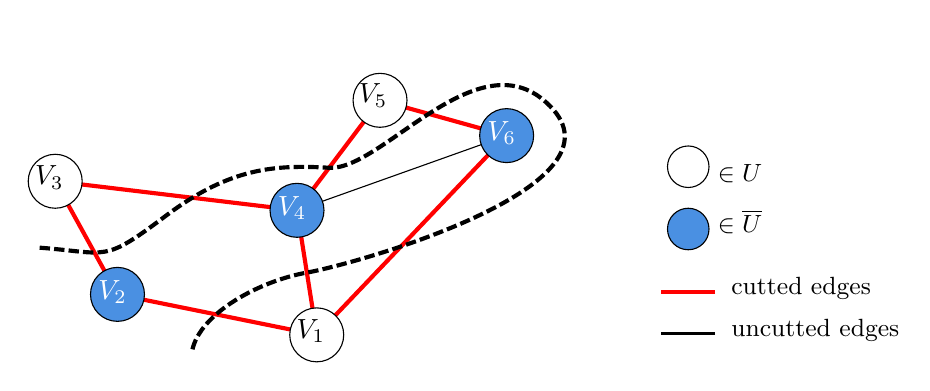
\begin{tikzpicture}[x=0.75pt,y=0.75pt,yscale=-1,xscale=1]
%uncomment if require: \path (0,159); %set diagram left start at 0, and has height of 159

%Straight Lines [id:da11964796995332005] 
\draw    (158.5,73.5) -- (259.5,37.5) ;
%Straight Lines [id:da15972910359553594] 
\draw [color={rgb, 255:red, 255; green, 0; blue, 0 }  ,draw opacity=1 ][line width=1.5]    (158.5,73.5) -- (168,133.5) ;
%Straight Lines [id:da2798044521653187] 
\draw [color={rgb, 255:red, 255; green, 0; blue, 0 }  ,draw opacity=1 ][line width=1.5]    (259.5,37.5) -- (198.5,20.5) ;
%Straight Lines [id:da7169631782552711] 
\draw [color={rgb, 255:red, 255; green, 0; blue, 0 }  ,draw opacity=1 ][line width=1.5]    (158.5,73.5) -- (198.5,20.5) ;
%Straight Lines [id:da026668841375865227] 
\draw [color={rgb, 255:red, 255; green, 0; blue, 0 }  ,draw opacity=1 ][line width=1.5]    (168,133.5) -- (259.5,37.5) ;
%Straight Lines [id:da10247267579193942] 
\draw [color={rgb, 255:red, 255; green, 0; blue, 0 }  ,draw opacity=1 ][line width=1.5]    (158.5,73.5) -- (42,59.5) ;
%Straight Lines [id:da6325731661518962] 
\draw [color={rgb, 255:red, 255; green, 0; blue, 0 }  ,draw opacity=1 ][line width=1.5]    (168,133.5) -- (72,114) ;
%Straight Lines [id:da6714305559976217] 
\draw [color={rgb, 255:red, 255; green, 0; blue, 0 }  ,draw opacity=1 ][line width=1.5]    (72,114) -- (42,59.5) ;
%Shape: Ellipse [id:dp9445310521915122] 
\draw  [fill={rgb, 255:red, 74; green, 144; blue, 226 }  ,fill opacity=1 ] (246.5,37.5) .. controls (246.5,30.32) and (252.32,24.5) .. (259.5,24.5) .. controls (266.68,24.5) and (272.5,30.32) .. (272.5,37.5) .. controls (272.5,44.68) and (266.68,50.5) .. (259.5,50.5) .. controls (252.32,50.5) and (246.5,44.68) .. (246.5,37.5) -- cycle ;
%Shape: Ellipse [id:dp5491993786197626] 
\draw  [fill={rgb, 255:red, 255; green, 255; blue, 255 }  ,fill opacity=1 ] (29,59.5) .. controls (29,52.32) and (34.82,46.5) .. (42,46.5) .. controls (49.18,46.5) and (55,52.32) .. (55,59.5) .. controls (55,66.68) and (49.18,72.5) .. (42,72.5) .. controls (34.82,72.5) and (29,66.68) .. (29,59.5) -- cycle ;
%Curve Lines [id:da8424711661169174] 
\draw [line width=1.5]  [dash pattern={on 3.75pt off 1.5pt}]  (34.5,91.5) .. controls (68,94) and (64.56,99.23) .. (95.5,76) .. controls (126.44,52.77) and (148,51.5) .. (174,53) .. controls (200,54.5) and (248,-13.5) .. (281.92,24.92) .. controls (315.83,63.33) and (185.58,99.58) .. (163.25,103.5) .. controls (140.92,107.42) and (111.42,122.92) .. (107.92,141.42) ;
%Shape: Ellipse [id:dp8814510692429732] 
\draw  [fill={rgb, 255:red, 255; green, 255; blue, 255 }  ,fill opacity=1 ] (337,52.5) .. controls (337,46.98) and (341.48,42.5) .. (347,42.5) .. controls (352.52,42.5) and (357,46.98) .. (357,52.5) .. controls (357,58.02) and (352.52,62.5) .. (347,62.5) .. controls (341.48,62.5) and (337,58.02) .. (337,52.5) -- cycle ;
%Shape: Ellipse [id:dp47339460639922903] 
\draw  [color={rgb, 255:red, 0; green, 0; blue, 0 }  ,draw opacity=1 ][fill={rgb, 255:red, 74; green, 144; blue, 226 }  ,fill opacity=1 ] (337,82.5) .. controls (337,76.98) and (341.48,72.5) .. (347,72.5) .. controls (352.52,72.5) and (357,76.98) .. (357,82.5) .. controls (357,88.02) and (352.52,92.5) .. (347,92.5) .. controls (341.48,92.5) and (337,88.02) .. (337,82.5) -- cycle ;
%Straight Lines [id:da23538055750108888] 
\draw [color={rgb, 255:red, 255; green, 0; blue, 0 }  ,draw opacity=1 ][line width=1.5]    (359.92,113) -- (334,113) ;
\draw [color={rgb, 255:red, 0; green, 0; blue, 0 }  ,draw opacity=1 ][line width=1.0]    (359.92,133) -- (334,133) ;
%Shape: Ellipse [id:dp4410323283239628] 
\draw  [fill={rgb, 255:red, 255; green, 255; blue, 255 }  ,fill opacity=1 ] (185.5,20.5) .. controls (185.5,13.32) and (191.32,7.5) .. (198.5,7.5) .. controls (205.68,7.5) and (211.5,13.32) .. (211.5,20.5) .. controls (211.5,27.68) and (205.68,33.5) .. (198.5,33.5) .. controls (191.32,33.5) and (185.5,27.68) .. (185.5,20.5) -- cycle ;
%Shape: Ellipse [id:dp23920294173784062] 
\draw  [fill={rgb, 255:red, 74; green, 144; blue, 226 }  ,fill opacity=1 ] (145.5,73.5) .. controls (145.5,66.32) and (151.32,60.5) .. (158.5,60.5) .. controls (165.68,60.5) and (171.5,66.32) .. (171.5,73.5) .. controls (171.5,80.68) and (165.68,86.5) .. (158.5,86.5) .. controls (151.32,86.5) and (145.5,80.68) .. (145.5,73.5) -- cycle ;
%Shape: Ellipse [id:dp6646352421974419] 
\draw  [fill={rgb, 255:red, 255; green, 255; blue, 255 }  ,fill opacity=1 ] (155,133.5) .. controls (155,126.32) and (160.82,120.5) .. (168,120.5) .. controls (175.18,120.5) and (181,126.32) .. (181,133.5) .. controls (181,140.68) and (175.18,146.5) .. (168,146.5) .. controls (160.82,146.5) and (155,140.68) .. (155,133.5) -- cycle ;
%Shape: Ellipse [id:dp5494896623298657] 
\draw  [fill={rgb, 255:red, 74; green, 144; blue, 226 }  ,fill opacity=1 ] (59,114) .. controls (59,106.82) and (64.82,101) .. (72,101) .. controls (79.18,101) and (85,106.82) .. (85,114) .. controls (85,121.18) and (79.18,127) .. (72,127) .. controls (64.82,127) and (59,121.18) .. (59,114) -- cycle ;

% Text Node
\draw (31,50.9) node [anchor=north west][inner sep=0.75pt]  [font=\normalsize]  {$V_{3}$};
% Text Node
\draw (360,50) node [anchor=north west][inner sep=0.75pt]  [font=\small]  {$\in U$};
% Text Node
\draw (360,72) node [anchor=north west][inner sep=0.75pt]  [font=\small]  {$\in \overline{U}$};
% Text Node
\draw (366.5,104.5) node [anchor=north west][inner sep=0.75pt]  [font=\small] [align=left] {cutted edges};
\draw (366.5,124.5) node [anchor=north west][inner sep=0.75pt]  [font=\small] [align=left] {uncutted edges};
% Text Node
\draw (187,11.4) node [anchor=north west][inner sep=0.75pt]  [font=\normalsize]  {$V_{5}$};
% Text Node
\draw (249,29.4) node [anchor=north west][inner sep=0.75pt]  [font=\normalsize,color={rgb, 255:red, 255; green, 255; blue, 255 }  ,opacity=1 ]  {$V_{6}$};
% Text Node
\draw (148,65.4) node [anchor=north west][inner sep=0.75pt]  [font=\normalsize,color={rgb, 255:red, 255; green, 255; blue, 255 }  ,opacity=1 ]  {$V_{4}$};
% Text Node
\draw (157,124.9) node [anchor=north west][inner sep=0.75pt]  [font=\normalsize]  {$V_{1}$};
% Text Node
\draw (61.5,105.9) node [anchor=north west][inner sep=0.75pt]  [font=\normalsize,color={rgb, 255:red, 255; green, 255; blue, 255 }  ,opacity=1 ]  {$V_{2}$};


\end{tikzpicture}

    \caption{An example of Maximum Cut problem. The dashed line cuts the seven edges that are highlighted in red. Consequently, the vertices are marked with different colors to indicate their belonging to partition $U$ or $\bar{U}$.}
    \label{fig:demo-max-cut}
\end{figure}



\begin{table}
\centering
\begin{tblr}{colspec={Q[c,h]cccc},stretch=0,rowsep=6pt}
\hline
spin indexing&N&label&sign of $J_k$&$\theta$\\\hline
\SetCell[r=3]{m} \scalebox{0.6}{

% Gradient Info
  
\tikzset {_q6d1jly0c/.code = {\pgfsetadditionalshadetransform{ \pgftransformshift{\pgfpoint{-7.5 bp } { 0 bp }  }  \pgftransformrotate{-225 }  \pgftransformscale{2 }  }}}
\pgfdeclarehorizontalshading{_0bsmz13ng}{150bp}{rgb(0bp)=(0.03,0.22,0.4);
rgb(37.5bp)=(0.03,0.22,0.4);
rgb(62.5bp)=(0,0.29,0.51);
rgb(100bp)=(0,0.29,0.51)}

% Gradient Info
  
\tikzset {_uvoxzm524/.code = {\pgfsetadditionalshadetransform{ \pgftransformshift{\pgfpoint{-7.5 bp } { 0 bp }  }  \pgftransformrotate{-225 }  \pgftransformscale{2 }  }}}
\pgfdeclarehorizontalshading{_fyest5jbo}{150bp}{rgb(0bp)=(0.03,0.22,0.4);
rgb(37.5bp)=(0.03,0.22,0.4);
rgb(62.5bp)=(0,0.29,0.51);
rgb(100bp)=(0,0.29,0.51)}

% Gradient Info
  
\tikzset {_py27uv7b1/.code = {\pgfsetadditionalshadetransform{ \pgftransformshift{\pgfpoint{-7.5 bp } { 0 bp }  }  \pgftransformrotate{-225 }  \pgftransformscale{2 }  }}}
\pgfdeclarehorizontalshading{_e66njv4ua}{150bp}{rgb(0bp)=(0.03,0.22,0.4);
rgb(37.5bp)=(0.03,0.22,0.4);
rgb(62.5bp)=(0,0.29,0.51);
rgb(100bp)=(0,0.29,0.51)}
\tikzset{every picture/.style={line width=0.75pt}} %set default line width to 0.75pt        


\begin{tikzpicture}[x=0.75pt,y=0.75pt,yscale=-1,xscale=1]
%uncomment if require: \path (0,141); %set diagram left start at 0, and has height of 141

%Shape: Square [id:dp40205531904810266] 
\draw  [draw opacity=0][shading=_0bsmz13ng,_q6d1jly0c] (120.31,35) -- (155.66,70.35) -- (120.31,105.71) -- (84.95,70.35) -- cycle ;
%Shape: Circle [id:dp6654608173556106] 
\draw   (113.24,13.78) .. controls (117.14,9.88) and (123.47,9.88) .. (127.38,13.78) .. controls (131.28,17.69) and (131.28,24.02) .. (127.38,27.92) .. controls (123.47,31.83) and (117.14,31.83) .. (113.24,27.92) .. controls (109.33,24.02) and (109.33,17.69) .. (113.24,13.78) -- cycle ;
%Shape: Circle [id:dp06811511385885272] 
\draw   (162.74,63.28) .. controls (166.64,59.37) and (172.97,59.37) .. (176.88,63.28) .. controls (180.78,67.19) and (180.78,73.52) .. (176.88,77.42) .. controls (172.97,81.33) and (166.64,81.33) .. (162.74,77.42) .. controls (158.83,73.52) and (158.83,67.19) .. (162.74,63.28) -- cycle ;
%Shape: Circle [id:dp866496050161264] 
\draw   (212.23,112.78) .. controls (216.14,108.87) and (222.47,108.87) .. (226.37,112.78) .. controls (230.28,116.68) and (230.28,123.01) .. (226.37,126.92) .. controls (222.47,130.82) and (216.14,130.82) .. (212.23,126.92) .. controls (208.33,123.01) and (208.33,116.68) .. (212.23,112.78) -- cycle ;
%Shape: Circle [id:dp8486257980974814] 
\draw   (63.74,63.28) .. controls (67.65,59.37) and (73.98,59.37) .. (77.88,63.28) .. controls (81.79,67.19) and (81.79,73.52) .. (77.88,77.42) .. controls (73.98,81.33) and (67.65,81.33) .. (63.74,77.42) .. controls (59.83,73.52) and (59.83,67.19) .. (63.74,63.28) -- cycle ;
%Shape: Circle [id:dp6621158362166136] 
\draw   (113.24,112.78) .. controls (117.14,108.87) and (123.47,108.87) .. (127.38,112.78) .. controls (131.28,116.68) and (131.28,123.01) .. (127.38,126.92) .. controls (123.47,130.82) and (117.14,130.82) .. (113.24,126.92) .. controls (109.33,123.01) and (109.33,116.68) .. (113.24,112.78) -- cycle ;
%Shape: Circle [id:dp9693194383410402] 
\draw   (14.24,112.78) .. controls (18.15,108.87) and (24.48,108.87) .. (28.38,112.78) .. controls (32.29,116.68) and (32.29,123.01) .. (28.38,126.92) .. controls (24.48,130.82) and (18.15,130.82) .. (14.24,126.92) .. controls (10.34,123.01) and (10.34,116.68) .. (14.24,112.78) -- cycle ;
%Shape: Right Triangle [id:dp28578880257729367] 
\draw  [draw opacity=0][shading=_fyest5jbo,_uvoxzm524] (105.92,120.1) -- (35.71,120.6) -- (71.06,85.24) -- cycle ;
%Shape: Right Triangle [id:dp9982201862645094] 
\draw  [draw opacity=0][shading=_e66njv4ua,_py27uv7b1] (205.16,119.85) -- (134.45,119.85) -- (169.81,84.49) -- cycle ;

% Text Node
\draw (115,14) node [anchor=north west][inner sep=0.75pt]   [align=left] {1};
% Text Node
\draw (66,63) node [anchor=north west][inner sep=0.75pt]   [align=left] {2};
% Text Node
\draw (165,63) node [anchor=north west][inner sep=0.75pt]   [align=left] {3};
% Text Node
\draw (16,113) node [anchor=north west][inner sep=0.75pt]   [align=left] {4};
% Text Node
\draw (115,113) node [anchor=north west][inner sep=0.75pt]   [align=left] {5};
% Text Node
\draw (214,113) node [anchor=north west][inner sep=0.75pt]   [align=left] {6};

\end{tikzpicture}} & \SetCell[r=3]{m} 6 
    & LHZ6E & $[+,+,-,-,+,-]$ &0.0 \\\hline
&   & \textbf{LHZ6M} & $[-,-,-,+,-,+]$ & 0.3\\\hline
&   & LHZ6H & $[+,+,+,-,-,+]$ & 0.55\\\hline
\hspace{-3mm}\scalebox{0.6}{

% Gradient Info
  
\tikzset {_2xhcrefu0/.code = {\pgfsetadditionalshadetransform{ \pgftransformshift{\pgfpoint{-7.5 bp } { 0 bp }  }  \pgftransformrotate{-225 }  \pgftransformscale{2 }  }}}
\pgfdeclarehorizontalshading{_spn6ydpdw}{150bp}{rgb(0bp)=(0.03,0.22,0.4);
rgb(37.5bp)=(0.03,0.22,0.4);
rgb(62.5bp)=(0,0.29,0.51);
rgb(100bp)=(0,0.29,0.51)}

% Gradient Info
  
\tikzset {_kw0p3luhv/.code = {\pgfsetadditionalshadetransform{ \pgftransformshift{\pgfpoint{-7.5 bp } { 0 bp }  }  \pgftransformrotate{-225 }  \pgftransformscale{2 }  }}}
\pgfdeclarehorizontalshading{_zquv02ocj}{150bp}{rgb(0bp)=(0.03,0.22,0.4);
rgb(37.5bp)=(0.03,0.22,0.4);
rgb(62.5bp)=(0,0.29,0.51);
rgb(100bp)=(0,0.29,0.51)}

% Gradient Info
  
\tikzset {_5nlio4lhy/.code = {\pgfsetadditionalshadetransform{ \pgftransformshift{\pgfpoint{-7.5 bp } { 0 bp }  }  \pgftransformrotate{-225 }  \pgftransformscale{2 }  }}}
\pgfdeclarehorizontalshading{_0px9iulda}{150bp}{rgb(0bp)=(0.03,0.22,0.4);
rgb(37.5bp)=(0.03,0.22,0.4);
rgb(62.5bp)=(0,0.29,0.51);
rgb(100bp)=(0,0.29,0.51)}

% Gradient Info
  
\tikzset {_i9m56ow0g/.code = {\pgfsetadditionalshadetransform{ \pgftransformshift{\pgfpoint{-7.5 bp } { 0 bp }  }  \pgftransformrotate{-225 }  \pgftransformscale{2 }  }}}
\pgfdeclarehorizontalshading{_cp2s0duqo}{150bp}{rgb(0bp)=(0.03,0.22,0.4);
rgb(37.5bp)=(0.03,0.22,0.4);
rgb(62.5bp)=(0,0.29,0.51);
rgb(100bp)=(0,0.29,0.51)}

% Gradient Info
  
\tikzset {_i0ciopkoo/.code = {\pgfsetadditionalshadetransform{ \pgftransformshift{\pgfpoint{-7.5 bp } { 0 bp }  }  \pgftransformrotate{-225 }  \pgftransformscale{2 }  }}}
\pgfdeclarehorizontalshading{_pfe2kjcao}{150bp}{rgb(0bp)=(0.03,0.22,0.4);
rgb(37.5bp)=(0.03,0.22,0.4);
rgb(62.5bp)=(0,0.29,0.51);
rgb(100bp)=(0,0.29,0.51)}

% Gradient Info
  
\tikzset {_4zjqptm1s/.code = {\pgfsetadditionalshadetransform{ \pgftransformshift{\pgfpoint{-7.5 bp } { 0 bp }  }  \pgftransformrotate{-225 }  \pgftransformscale{2 }  }}}
\pgfdeclarehorizontalshading{_2wsugf3gc}{150bp}{rgb(0bp)=(0.03,0.22,0.4);
rgb(37.5bp)=(0.03,0.22,0.4);
rgb(62.5bp)=(0,0.29,0.51);
rgb(100bp)=(0,0.29,0.51)}
\tikzset{every picture/.style={line width=0.75pt}} %set default line width to 0.75pt        

\begin{tikzpicture}[x=0.75pt,y=0.75pt,yscale=-1,xscale=1]
%uncomment if require: \path (0,184); %set diagram left start at 0, and has height of 184

%Shape: Square [id:dp4646069098280107] 
\draw  [draw opacity=0][shading=_spn6ydpdw,_2xhcrefu0] (166.72,29.33) -- (202.08,64.68) -- (166.72,100.04) -- (131.36,64.68) -- cycle ;
%Shape: Circle [id:dp1768374451497594] 
\draw   (159.65,8.11) .. controls (163.55,4.21) and (169.89,4.21) .. (173.79,8.11) .. controls (177.7,12.02) and (177.7,18.35) .. (173.79,22.26) .. controls (169.89,26.16) and (163.55,26.16) .. (159.65,22.26) .. controls (155.74,18.35) and (155.74,12.02) .. (159.65,8.11) -- cycle ;
%Shape: Circle [id:dp9515478681131959] 
\draw   (209.15,57.61) .. controls (213.05,53.71) and (219.38,53.71) .. (223.29,57.61) .. controls (227.19,61.52) and (227.19,67.85) .. (223.29,71.75) .. controls (219.38,75.66) and (213.05,75.66) .. (209.15,71.75) .. controls (205.24,67.85) and (205.24,61.52) .. (209.15,57.61) -- cycle ;
%Shape: Circle [id:dp7756495234805515] 
\draw   (258.64,107.11) .. controls (262.55,103.2) and (268.88,103.2) .. (272.79,107.11) .. controls (276.69,111.01) and (276.69,117.35) .. (272.79,121.25) .. controls (268.88,125.16) and (262.55,125.16) .. (258.64,121.25) .. controls (254.74,117.35) and (254.74,111.01) .. (258.64,107.11) -- cycle ;
%Shape: Circle [id:dp2733517995597814] 
\draw   (110.15,57.61) .. controls (114.06,53.71) and (120.39,53.71) .. (124.29,57.61) .. controls (128.2,61.52) and (128.2,67.85) .. (124.29,71.75) .. controls (120.39,75.66) and (114.06,75.66) .. (110.15,71.75) .. controls (106.25,67.85) and (106.25,61.52) .. (110.15,57.61) -- cycle ;
%Shape: Circle [id:dp7014226103914162] 
\draw   (159.65,107.11) .. controls (163.55,103.2) and (169.89,103.2) .. (173.79,107.11) .. controls (177.7,111.01) and (177.7,117.35) .. (173.79,121.25) .. controls (169.89,125.16) and (163.55,125.16) .. (159.65,121.25) .. controls (155.74,117.35) and (155.74,111.01) .. (159.65,107.11) -- cycle ;
%Shape: Circle [id:dp07847046561305948] 
\draw   (60.65,107.11) .. controls (64.56,103.2) and (70.89,103.2) .. (74.8,107.11) .. controls (78.7,111.01) and (78.7,117.35) .. (74.8,121.25) .. controls (70.89,125.16) and (64.56,125.16) .. (60.65,121.25) .. controls (56.75,117.35) and (56.75,111.01) .. (60.65,107.11) -- cycle ;
%Shape: Right Triangle [id:dp18543834280062976] 
\draw  [draw opacity=0][shading=_zquv02ocj,_kw0p3luhv] (202.08,164.18) -- (131.36,164.18) -- (166.72,128.82) -- cycle ;
%Shape: Right Triangle [id:dp019748006978987376] 
\draw  [draw opacity=0][shading=_0px9iulda,_5nlio4lhy] (300.82,163.93) -- (230.61,164.43) -- (265.97,129.07) -- cycle ;
%Shape: Circle [id:dp3946162772039473] 
\draw   (209.15,156.61) .. controls (213.05,152.7) and (219.38,152.7) .. (223.29,156.61) .. controls (227.19,160.51) and (227.19,166.84) .. (223.29,170.75) .. controls (219.38,174.65) and (213.05,174.65) .. (209.15,170.75) .. controls (205.24,166.84) and (205.24,160.51) .. (209.15,156.61) -- cycle ;
%Shape: Circle [id:dp6620738247447955] 
\draw   (110.15,156.61) .. controls (114.06,152.7) and (120.39,152.7) .. (124.29,156.61) .. controls (128.2,160.51) and (128.2,166.84) .. (124.29,170.75) .. controls (120.39,174.65) and (114.06,174.65) .. (110.15,170.75) .. controls (106.25,166.84) and (106.25,160.51) .. (110.15,156.61) -- cycle ;
%Shape: Circle [id:dp027305429094700795] 
\draw   (11.16,156.61) .. controls (15.06,152.7) and (21.39,152.7) .. (25.3,156.61) .. controls (29.2,160.51) and (29.2,166.84) .. (25.3,170.75) .. controls (21.39,174.65) and (15.06,174.65) .. (11.16,170.75) .. controls (7.25,166.84) and (7.25,160.51) .. (11.16,156.61) -- cycle ;
%Shape: Circle [id:dp5838580222665838] 
\draw   (308.14,156.61) .. controls (312.05,152.7) and (318.38,152.7) .. (322.28,156.61) .. controls (326.19,160.51) and (326.19,166.84) .. (322.28,170.75) .. controls (318.38,174.65) and (312.05,174.65) .. (308.14,170.75) .. controls (304.24,166.84) and (304.24,160.51) .. (308.14,156.61) -- cycle ;
%Shape: Right Triangle [id:dp051990486144260606] 
\draw  [draw opacity=0][shading=_cp2s0duqo,_i9m56ow0g] (102.83,163.93) -- (32.62,164.43) -- (67.98,129.07) -- cycle ;
%Shape: Square [id:dp556944438890764] 
\draw  [draw opacity=0][shading=_pfe2kjcao,_i0ciopkoo] (216.22,78.82) -- (251.57,114.18) -- (216.22,149.53) -- (180.86,114.18) -- cycle ;
%Shape: Square [id:dp31466343787367357] 
\draw  [draw opacity=0][shading=_2wsugf3gc,_4zjqptm1s] (117.22,78.82) -- (152.58,114.18) -- (117.22,149.53) -- (81.87,114.18) -- cycle ;

% Text Node
\draw (162,8) node [anchor=north west][inner sep=0.75pt]   [align=left] {1};
% Text Node
\draw (112,58) node [anchor=north west][inner sep=0.75pt]   [align=left] {2};
% Text Node
\draw (211,58) node [anchor=north west][inner sep=0.75pt]   [align=left] {3};
% Text Node
\draw (62,107) node [anchor=north west][inner sep=0.75pt]   [align=left] {4};
% Text Node
\draw (162,107) node [anchor=north west][inner sep=0.75pt]   [align=left] {5};
% Text Node
\draw (260,107) node [anchor=north west][inner sep=0.75pt]   [align=left] {6};
% Text Node
\draw (13,157) node [anchor=north west][inner sep=0.75pt]   [align=left] {7};
% Text Node
\draw (112,157) node [anchor=north west][inner sep=0.75pt]   [align=left] {8};
% Text Node
\draw (211,157) node [anchor=north west][inner sep=0.75pt]   [align=left] {9};
% Text Node
\draw (306,157) node [anchor=north west][inner sep=0.75pt]   [align=left] {10};


\end{tikzpicture}
} & 10 & LHZ10&\makecell{$[-,-,-,-,+$\\$\;\;+,+,-,-,-]$}&0.3\\
\hline
\end{tblr}
    \caption{\label{tab:demo-draw} Selected instances of LHZ models that are considered in the following analysis. The constraints are fixed to $C_l=-2$ and the magnitude of the local fields to $|J_k|=1$. The signs of $J_k$ that fully determine the instance are reported in the table, along with the label of the instance and its ``hardness'' $\theta$. The reference study case is LHZ6M.}
\end{table}

